\chapter{Wstęp}

\section{Cel pracy}
\begin{par}
	Celem ninejszej pracy inżynierskiej jest stworzenie silnika dynamiki brył
	sztywnych działającego w czasie rzeczywistym, który mógłby być wykorzystywany
	do symulacji fizycznych na potrzeby gier komputerowych. Oznacza to między
	innymi, że efekty pracy silnika powinny raczej wyglądać wiarygodnie, niż
	skupiać się na dokładnym odwzorowaniu zjawisk fizycznych. Dlatego wystarczający
	jest uproszczony model fizyczny. Z drugiej strony silnik musi radzić sobie z
	symulacją dużej liczby obiektów równocześnie w czasie rzeczywistym, czyli
	znając stan świata dla chwili $T$, musi wyliczyć stan świata dla chwili
	$T+\Delta{}T$ w czasie rzeczywistym nie dłuższym niż $\Delta{}T$.
\end{par} \\
\begin{par}
	Dodatkowym celem pracy jest poszerzenie wiedzy o silnikach
	fizycznych, poprzez zbadanie możliwości silników obecnie istniejących, oraz
	poprzez porównanie ich z właściwościami silnika tworzonego w ramach tej pracy
	inżynierskiej. Jest to o tyle ważne, że ninejsza praca proponuje innowacyjny
	sposób obliczania właściwości fizycznych oraz wykrywania kolizji między
	obiektami oparty o wypełnienie obiektów Kisielkami\footnote{\ pojęcie
	wyjaśnione w następnej sekcji --- `Definicje pojęć`}.
\end{par} \\
\begin{par}
	Celem pobocznym pracy jest również stworzenie przykładowej aplikacji lub
	prostej gry prezentującej możliwości silnika, aby umożliwić przyszłym
	użytkownikom, oraz innym osobom zainteresowanym naszym silnikiem, szybkie i
	łatwe zapoznanie się ze sposobem wykorzystania silnika oraz oferowaną przez niego funkcjonalnością.
\end{par}

\section{Definicje pojęć}
\begin{itemize}
  \item Kisielek --- cząstka dyskretna, przybliżająca masę i objętość swojego
	najbliższego otoczenia. Pojedynczy obiekt fizyczny może się składać z dowolnie
	dużej, ale skończonej, liczby Kisielków. Kisielki pojedynczego obiektu nie
	przemieszczają się względem siebie (wg. definicji bryły sztywnej). Kolizje
	obiektów są rozpatrywane jako kolizje pomiędzy parami Kisielków danych
	obiektów.
	\item Kisielstwo --- podgrupa Kisielków pojedynczego obiektu. Obiekt fizyczny
	może być podzielony na wiele rozłącznych Kisielstw. Kisielki są grupowane w
	celu przyspieszenia wykrywania kolizji, poprzez wstępne rozpatrywanie kolizji między
	grupami Kisielków --- Kisielstwami.
	\item Podkisielstwo --- podgrupa Kisielków należących do pojedynczego
	Kisielstwa. Kisielki tworzą hierarchiczną strukturę, którą można
	przedstawić jako drzewo:
	\begin{figure}[!h]
		\centering
		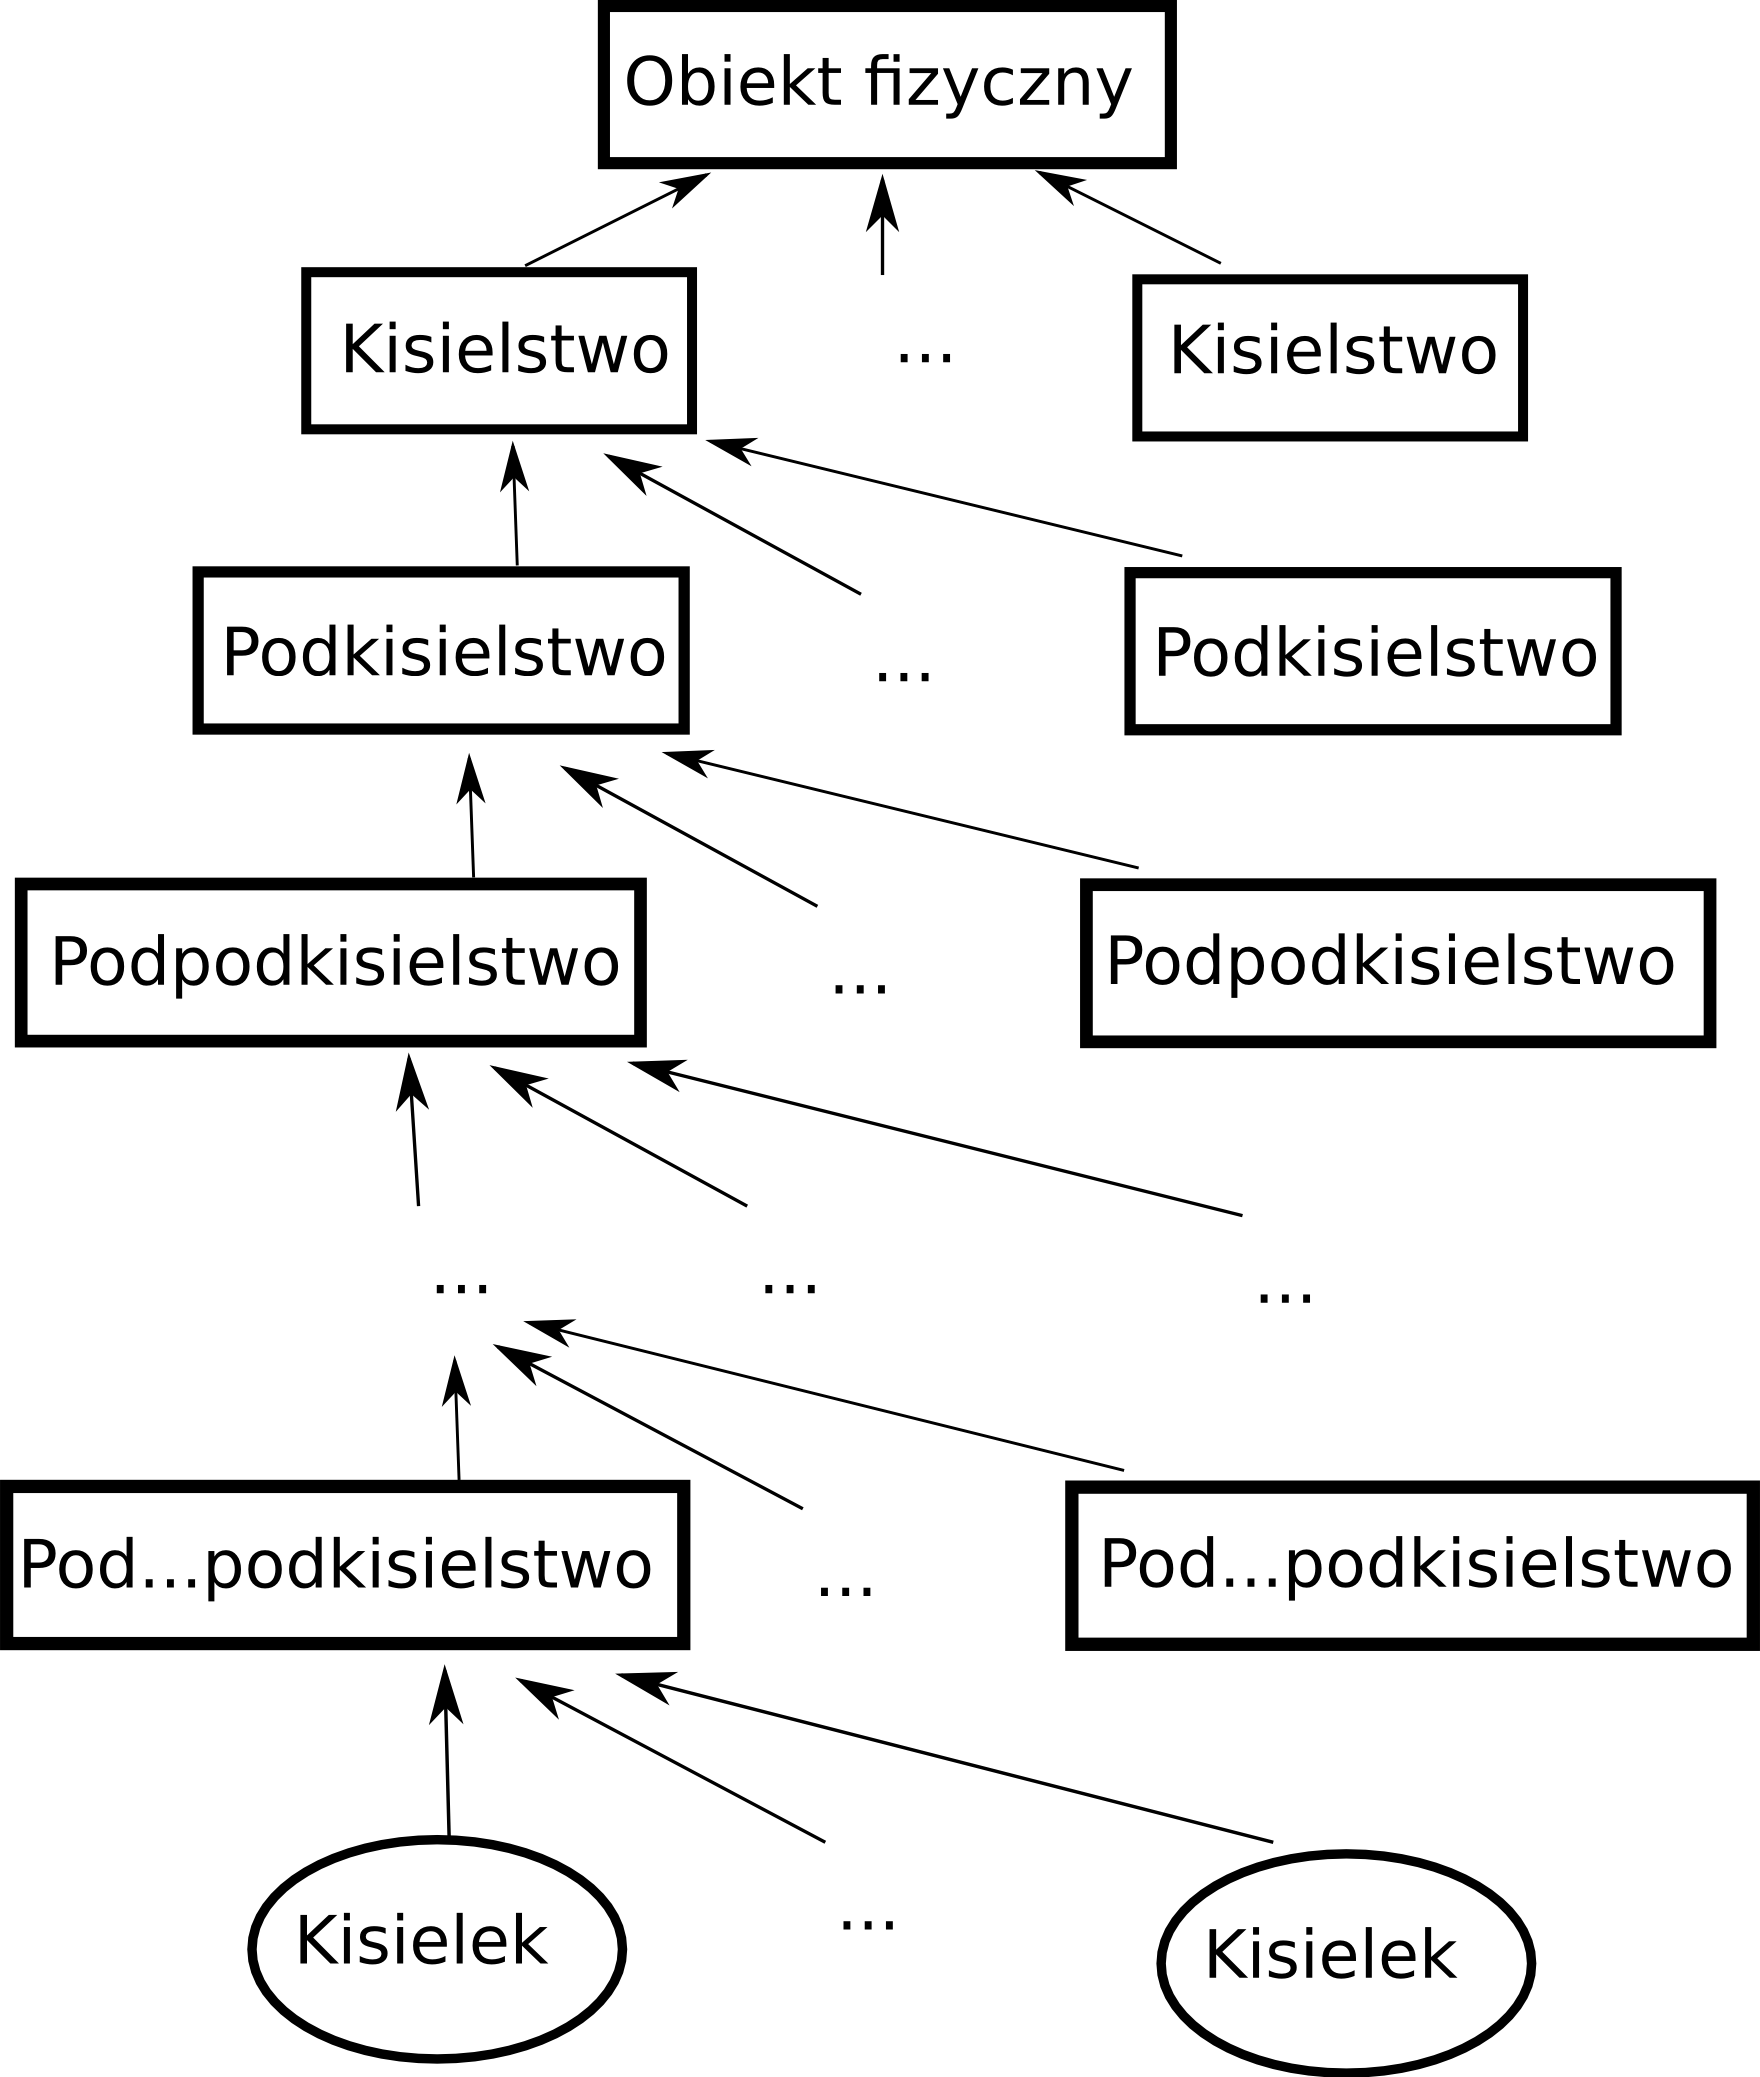
\includegraphics[height=90mm]{images/Hierarchia.png}
	\end{figure}
	\item Impuls --- momentalna zmiana pędu i momentu pędu obiektu np. na skutek
	kolizji. Jest to pojęcie stworzone w celu uniknięcia obliczania siły dążącej do
	nieskończoności przy czasie dążącym do zera, które by wynikło z założenia, że
	czas kolizji jest pomijalnie krótki.
	\item Wszechkisiel --- zarządca, pojedynczy na całą symulację obiekt, u którego
	użytkownik rejestruje informacje pomiędzy którymi obiektami mają być wykrywane
	kolizje, a pomiędzy którymi nie. Odpowiada również za stałe globalne (np.
	przyspieszenie grawitacyjne, długość kroku symulacji).
\end{itemize}

\section{Zadania do wykonania i podział pracy}
\begin{center}
	Implementacja
	\begin{longtable}{|p{30mm}|p{85mm}|p{8mm}|} \hline
	Kinematyka & zagadnienia związane z położeniem i orientacją obiektu oraz
	ich pochodnymi, w tym całkowanie numeryczne mające na celu wyliczenie
	kolejnego stanu obiektu & JR \\ \hline
	
	Kinetyka & obliczanie $m$, $I$, $\vec{F}$, $\vec{\tau}$, oraz ich wpływu na
	dynamikę obiektu & JR \\ \hline
	
	Relacje między obiektami & powiązania między obiektami, np. sprężyny, nacisk
	statyczny, obiekty sklejone ze sobą, zawiasy & JR \\ \hline
	
    Obsługa kolizji & metodą sprężyn-amortyzatorów & JR \\ \hline
    
    Rozpadanie się obiektów & reakcja niektórych obiektów na silne kolizje,
    skutkująca rozpadem na mniejsze obiekty & JR \\ \hline \hline
    
    Wypełnianie Kisielkami & algorytm wypełniający zadaną bryłę geometryczną
    Kisielkami i tworzący ich hierarchię & KB
    \\ \hline
    
    Algorytm podziału & dzielący obiekt na Kisielstwa i kolejne poziomy, w taki
    sposób, aby zoptymalizować późniejsze wykrywanie kolizji & KB
    \\ \hline
    
    Wykrywanie kolizji & pomiędzy kulami opisanymi na Kisielstwach, oraz
    pomiędzy kolejnymi poziomami hierarchii, aż do poszczególnych Kisielków & KB \\ \hline
    
    Obsługa kolizji & metodą impulsów & KB \\ \hline
    
    Zarządca (Wszechkisiel) & stworzenie obiektu zarządzającego wykrywaniem
    kolizji (grupy kolizyjne), oraz globalnymi parametrami silnika (np. grawitacja) & KB
    \\ \hline
    
	\end{longtable}
    
    Inne
	\begin{longtable}{|p{120mm}|p{8mm}|} \hline
    Tworzenie dokumentacji & JR \\ \hline
    Testy wydajnościowe & JR \\ \hline
    Przykładowa aplikacja demonstracyjna & JR \\ \hline \hline
    Opracowanie algorytmów & KB \\ \hline
    Wizualizacja wypełnienia Kisielkami & KB \\ \hline
	\end{longtable}
\end{center}

\newpage
\section{Harmonogram}
	Faza analizy i projektowania
	\begin{longtable}{|p{85mm}|p{42mm}|} \hline
	
    Zapoznanie się z istniejącymi silnikami fizycznymi &
    1.10.2011 -- 15.10.2011
    \\ \hline
    
    Przeczytanie "Fizyki dla programistów gier"\cite{pfgd} &
    1.10.2011 -- 1.11.2011
    \\ \hline
    
    Opracowanie algorytmów wykrywania kolizji, obsługi kolizji, wypełniania
    geometrii Kisielkami, całkowania numerycznego, oraz rozpadania się obiektów
    & 1.10.2011 -- 1.11.2011
    \\ \hline
    
    Implementacja prototypów na podstawie podręcznika\cite{pfgd} &
    15.10.2011 -- 1.11.2011
    \\ \hline
    
    Zaprojektowanie interfejsów poprzez które użytkownik będzie z silnika
    korzystał & 15.10.2011 -- 1.11.2011
    \\ \hline
    
    Zaprojektowanie interfejsów komunikacji pomiędzy poszczególnymi modułami
    silnika & 15.10.2011 -- 1.11.2011
    \\ \hline
    
    Zaprojektowanie architektury silnika &
    15.10.2011 -- 7.11.2011
    \\ \hline
    
	\end{longtable}
	
	Faza implementacji
	\begin{longtable}{|p{85mm}|p{42mm}|} \hline
	
    Implementacja kinematyki, kinetyki i wypełniania Kisielkami &
    1.11.2011 -- 15.11.2011
    \\ \hline
	
    Implementacja wykrywania kolizji, obsługi kolizji, oraz relacji między
    obiektami & 15.11.2011 -- 1.12.2011
    \\ \hline
	
    Implementacja aplikacji demonstracyjnej
    & 15.11.2011 -- 7.12.2011
    \\ \hline
	
    Implementacja rozpadania się obiektów, oraz zarządcy (Wszechkiśla)
    & 1.12.2011 -- 7.12.2011
    \\ \hline
    
	\end{longtable}
	
	Faza zakończeniowa
	\begin{longtable}{|p{85mm}|p{42mm}|} \hline
	
    Testy wydajnościowe i jakościowe &
    15.11.2011 -- 7.12.2011
    \\ \hline
	
    Opracowanie ostatecznej dokumentacji projektu i instrukcji obsługi
    & 15.11.2011 -- 7.12.2011
    \\ \hline
	
	Przygotowanie produktu do przekazania (spakowanie jako biblioteki, wraz z
	zależnościami, oraz dołączoną dokumentacją)
	& 1.12.2011 -- 7.12.2011
    \\ \hline
    
	\end{longtable}